\documentclass[ 12pt ]{article}
\usepackage{amsmath, amsthm, amssymb, csquotes, enumitem, graphicx, listings, mathrsfs}
\usepackage[margin=0.5in]{geometry}
\graphicspath{ ./ }

\begin{document}

\begin{titlepage}
    \begin{center}
        \vspace*{1cm}
            
        \LARGE
        \textbf{CS 479 Pattern Recognition}

        \vspace{0.5cm}
        \LARGE
        \textbf{Programming Assignment 3}

        \vspace{0.1cm}
        \LARGE
        \textbf{Dimensionality Reduction}
            
        \vspace{1.5cm}
            
        \textbf{Logan Leavitt \& Landon Fox}
            
        \vfill
        \Large
        \textbf{Collaboration}

        \vspace{0.1cm}
        \large
        For the implementation, both Logan and Landon contributed. Logan carried out the training and classification methods as well as experiments \textbf{b} and \textbf{d}.
        Landon worked on the image input/output in addition to experiments \textbf{a} and \textbf{c}. \\
        In regard to the report, Logan worked on the Results, formatting, and grammar. Landon contributed to the Theory and Implementation.
            
        \vspace{0.8cm}
            
            
        \Large
        University of Nevada Reno\\
        April 28, 2021
            
    \end{center}
\end{titlepage}


\section*{Theory}

\qquad Due to the \textit{Curse of Dimensionality}, it is often not the case that performance is increased with the number of parameters; in fact, it is often quite the opposite since the
number of required training data increases exponentially. The goal of dimensionality reduction is to reduce the number of dimensions to its optimum to increase performance.
\begin{center}
    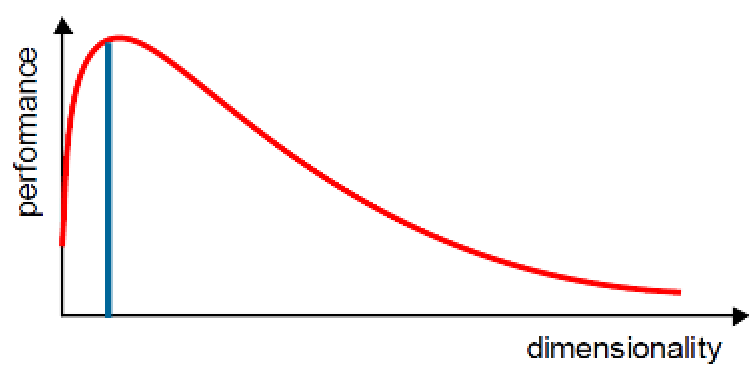
\includegraphics[scale=0.7]{optimum dim}
\end{center}
\begin{center}
    \scriptsize
    Figure 1: An average plot of a classifier's performance with respect to dimension.
\end{center}
Principal Component Analysis (PCA) is an approach to dimensionality reduction that attempts to approximate a feature $\textbf{x} \in \mathbb{R}^n$ by projecting it to a subspace
$V \subseteq \mathbb{R}^n$ with dimension $k \in \mathbb{N}$, where $k$ is far less than $n$. Moreover, it seeks a minimal collection of $k$ vectors, $\textbf{u}_1, \textbf{u}_2, \hdots,
\textbf{u}_k$, such that the subspace $$V = \mathrm{span}\{ \textbf{u}_1, \textbf{u}_2, \hdots, \textbf{u}_k \}$$ minimizes $$\min_{\widehat{\textbf{x}} \in V}\, \lVert \textbf{x} -
\widehat{\textbf{x}} \rVert,$$ informational loss. When provided samples features, the algorithm for PCA is as follows:
\begin{enumerate}
    \item Compute the covariance matrix of the provided data as well as its eigenvalues and eigenvectors. Center the data at the origin if possible.
    \item Select the $k$ eigenvectors associated with the $k$ largest eigenvalues. This will act as the basis of our subspace.
    \item Project all features $\textbf{x}$ onto the newly created subspace of lower dimension. That is, compute $y_1, \hdots, y_k$ where $$\widehat{\textbf{x}} - \overline{\textbf{x}} =
        \sum_{i=1}^k y_i \textbf{u}_i$$ where $\textbf{u}_i$ for $1 \leq i \leq k$ is the computed eigenvectors.
\end{enumerate}
Do note that we may further simplify projections as a linear transformation for more efficient computations. The $k$ largest eigenvectors of the estimated covariance matrix are of strong
importance in this algorithm because the largest eigenvalues represent the most substantial variances in the distribution. Furthermore, the corresponding eigenvectors represent the
direction in which most data varies.  Additionally in regard to the subspace basis, we can guarantee that it will be orthogonal due to the symmetry of the covariance matrix, providing
independence as desired. Hence, PCA attempts to preserve as much information as possible in $k$ dimensions by discarding $n-k$ that vary little in comparison to others.

As illustrated above, the value $k$ is essential as it dictates the \textit{optimal} dimension for our model. When provided a threshold $0 \leq t \leq 1$, the percentage of information
preservation, we may define $k$ as the the minimal value satisfying $$\frac{\sum_{i=1}^k \lambda_i}{\sum_{i=1}^n \lambda_i} > t$$ where $\lambda_i$ are the eigenvalues of the covariance
matrix of dimension $n \times n$.

An application of dimensionality reduction is facial recognition. Often when classifying images, the pixels are unwrapped into a vector of dimension $n^2$ which may be very large and so
dimensionality reduction is of great importance. PCA can be applied directly with only a few modifications. Namely, when provided $m$ $n \times n$ images unwrapped to vectors of length
$n^2$, denoted $\mathbf{\Phi}_i$, the covariance matrix becomes $$\Sigma = \frac{1}{m} \sum_{i=1}^m \mathbf{\Phi}_i \mathbf{\Phi}_i^t = \frac{1}{m}AA^t$$ where $A = \left [
\mathbf{\Phi}_1 \hdots \mathbf{\Phi}_m \right ]$. Computing the eigenvalues and eigenvectors of an $n^2 \times n^2$ covariance matrix can be very expensive. Here, we may exploit the fact
that the $k$ largest eigenvalues and eigenvectors of $AA^t$ and $A^tA$, an $m \times m$ matrix, are shared. This allows us to compute the spectrum in a more computationally efficient
manner. Due to the fact that vectors represent images, eigenvectors are also images and so we may visually represent them. We will refer to these eigenvectors as \textit{eigenfaces}.
\begin{center}
    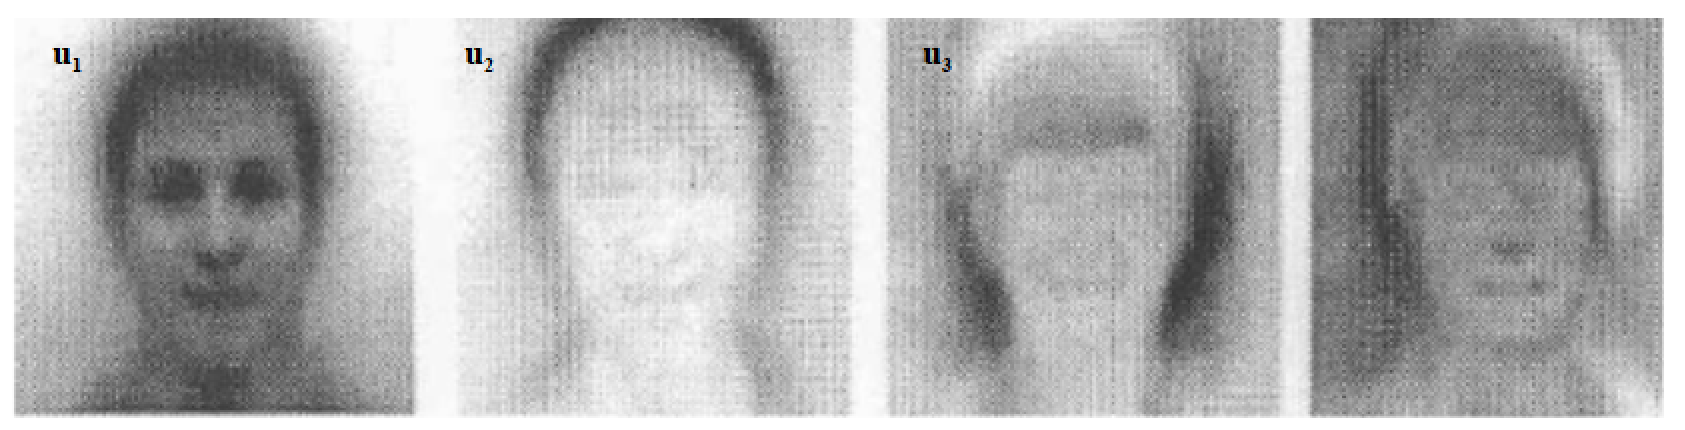
\includegraphics[scale=0.5]{eigenfaces}
    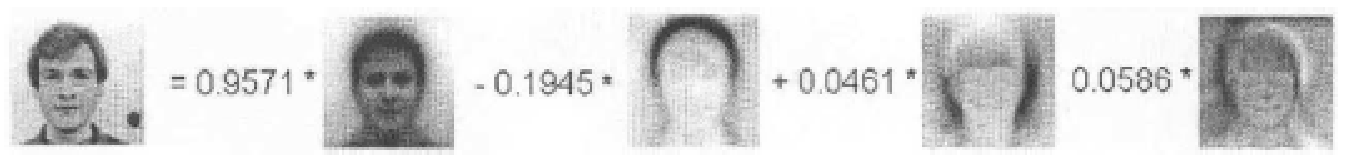
\includegraphics[scale=0.7]{eigenfaces_lc}
\end{center}
\begin{center}
    \scriptsize
    Figure 2: Examples of eigenfaces as well as a linear combination of eigenfaces.
\end{center}
One may use this approach to classify faces; when provided many images of an individual, one can train a model using these images and then classify new images of the individual
by finding training images \textit{nearest} to it. However, one downside to this approach is that all images must be normalized. That is, images must only contain their face and have
similar lighting and face orientation.


\section*{Implementation}

\qquad To implement PCA in the context of facial recognition, we utilized the \verb|Armadillo| C++ linear algebra library. This allowed us to perform vector and matrix arithmetic as well as
computing eigenvalues and eigenvectors. Similarly, for image input and output, we implemented the \verb|Image| class to perform the desired operations. Within the \verb|main| file, we
have the functions \verb|train| and \verb|classify| which will take a directory of images as input. The function \verb|train| when provided a collection of images will flatten them into
vectors, compute the covariance matrix as well as its eigenvalues and eigenvectors, then store all relevant information such as the eigenvalues and projection coefficients.
Correspondingly, when given an image and the projection coefficients computed by \verb|train|, \verb|classify| returns an array of images sorted with respect to the minimal Mahalanobis
distance from the provided image. With these functions, as well as some helper functions like \verb|flatten_image|, \verb|mahalanobis|, and \verb|truncate|, we are able to train our
classifier as well as test it by selecting the images nearest to it.


\section*{Results}

\begin{enumerate}
    \item[\textbf{a.}]
        \begin{enumerate}
            \item[\textbf{i.}] The average face as well as the ten largest and smallest eigenfaces are presented in Figures 3, 4, and 5, respectively, for the \verb|fa_H| collection.
                \begin{center}
                    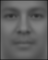
\includegraphics[scale=1.7]{AnyConv.com__average_face}
                \end{center}
                \begin{center}
                    \scriptsize
                    Figure 3: The average face of the \verb|fa_H| collection.
                \end{center}

                \begin{center}
                    
\includegraphics[scale=1.7]{AnyConv.com__largest1}
                    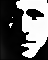
\includegraphics[scale=1.7]{AnyConv.com__largest2}
                    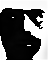
\includegraphics[scale=1.7]{AnyConv.com__largest3}
                    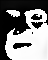
\includegraphics[scale=1.7]{AnyConv.com__largest4}
                    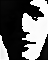
\includegraphics[scale=1.7]{AnyConv.com__largest5}
                    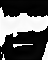
\includegraphics[scale=1.7]{AnyConv.com__largest6}
                    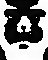
\includegraphics[scale=1.7]{AnyConv.com__largest7}
                    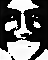
\includegraphics[scale=1.7]{AnyConv.com__largest8}
                    
\includegraphics[scale=1.7]{AnyConv.com__largest9}
                    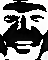
\includegraphics[scale=1.7]{AnyConv.com__largest10}
                \end{center}
                \begin{center}
                    \scriptsize
                    Figure 4: The eigenfaces corresponding to the ten largest eigenvalues of the \verb|fa_H| collection.
                \end{center}

                \begin{center}
                    
\includegraphics[scale=1.7]{AnyConv.com__smallest1}
                    
\includegraphics[scale=1.7]{AnyConv.com__smallest2}
                    
\includegraphics[scale=1.7]{AnyConv.com__smallest3}
                    
\includegraphics[scale=1.7]{AnyConv.com__smallest4}
                    
\includegraphics[scale=1.7]{AnyConv.com__smallest5}
                    
\includegraphics[scale=1.7]{AnyConv.com__smallest6}
                    
\includegraphics[scale=1.7]{AnyConv.com__smallest7}
                    
\includegraphics[scale=1.7]{AnyConv.com__smallest8}
                    
\includegraphics[scale=1.7]{AnyConv.com__smallest9}
                    
\includegraphics[scale=1.7]{AnyConv.com__smallest10}
                \end{center}
                \begin{center}
                    \scriptsize
                    Figure 5: The eigenfaces corresponding to the ten smallest eigenvalues of the \verb|fa_H| collection.
                \end{center}

            \item[\textbf{ii.}] Figure 6 illustrates the CMC curve when varying the number of images with the highest similarity scores between 1 and 50.
                \begin{center}
                    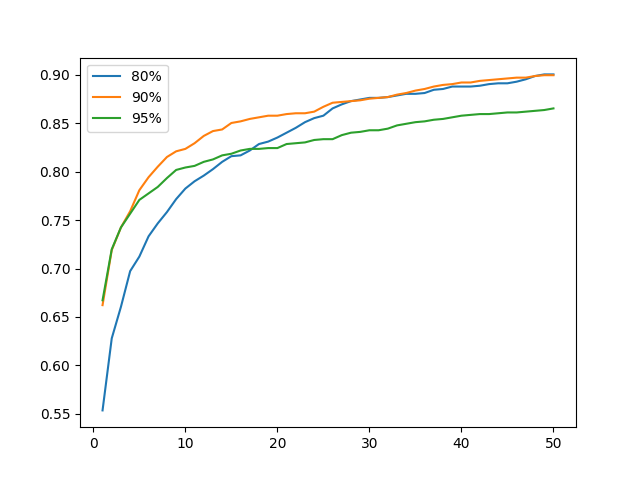
\includegraphics[scale=0.6]{cmc}
                \end{center}
                \begin{center}
                    \scriptsize
                    Figure 6: The CMC curve for the \verb|fb_H| collection.
                \end{center}

            \item[\textbf{iii.}] Assuming that we consider only one image with the highest similarity score, Figure 7 illustrates query images and their corresponding correct matches
                when preserving 80\% of all information.
                \begin{center}
                    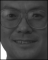
\includegraphics[scale=1.7]{f_h_images/AnyConv.com__00182_940422_fb_a}
                    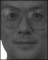
\includegraphics[scale=1.7]{f_h_images/AnyConv.com__00182_940422_fa_a}
                % \end{center}
                % \begin{center}
                    
\includegraphics[scale=1.7]{f_h_images/AnyConv.com__00753_941201_fb}
                    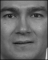
\includegraphics[scale=1.7]{f_h_images/AnyConv.com__00753_941201_fa}
                \end{center}
                \begin{center}
                    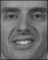
\includegraphics[scale=1.7]{f_h_images/AnyConv.com__00501_940519_fb}
                    
\includegraphics[scale=1.7]{f_h_images/AnyConv.com__00501_940519_fa}
                \end{center}
                \begin{center}
                    \scriptsize
                    Figure 7: Three query images and their correct corresponding matches from the \verb|fb_H| and \verb|fa_H| collections, respectively, with 80\%
                    information preservation.
                \end{center}

            \item[\textbf{iv.}] Again, only considering only one image with the highest similarity score, Figure 8 depicts query images incorrectly matched when preserving 80\% of all
                information.
                \newpage
                \begin{center}
                    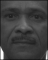
\includegraphics[scale=1.7]{f_h_images/AnyConv.com__00183_940128_fb}
                    
\includegraphics[scale=1.7]{f_h_images/AnyConv.com__00276_940422_fa_a}
                % \end{center}
                % \begin{center}
                    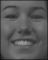
\includegraphics[scale=1.7]{f_h_images/AnyConv.com__00451_940422_fb}
                    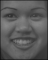
\includegraphics[scale=1.7]{f_h_images/AnyConv.com__00410_940422_fa}
                \end{center}
                \begin{center}
                    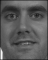
\includegraphics[scale=1.7]{f_h_images/AnyConv.com__00594_941031_fb}
                    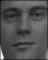
\includegraphics[scale=1.7]{f_h_images/AnyConv.com__00002_940128_fa}
                \end{center}
                \begin{center}
                    \scriptsize
                    Figure 8: Three query images and their incorrect matches from the \verb|fb_H| and \verb|fa_H| collections, respectively, with 80\% information
                    preservation.
                \end{center}

            \item[\textbf{v.}] Now we repeat the process with 90\% and 95\% information preservation. Figures 9 and 10 illustrate three correct and incorrect matchings, respectively,
                with both 90\% and 95\% data preservation. Indeed, after altering the data preservation from 90\% to 95\%, there was no modification to the returned matchings.
                \begin{center}
                    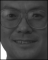
\includegraphics[scale=1.7]{f_h_images/AnyConv.com__00182_940422_fb_a}
                    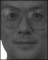
\includegraphics[scale=1.7]{f_h_images/AnyConv.com__00182_940422_fa_a}
                % \end{center}
                % \begin{center}
                    
\includegraphics[scale=1.7]{f_h_images/AnyConv.com__00753_941201_fb}
                    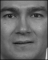
\includegraphics[scale=1.7]{f_h_images/AnyConv.com__00753_941201_fa}
                \end{center}
                \begin{center}
                    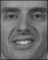
\includegraphics[scale=1.7]{f_h_images/AnyConv.com__00501_940519_fb}
                    
\includegraphics[scale=1.7]{f_h_images/AnyConv.com__00501_940519_fa}
                \end{center}
                \begin{center}
                    \scriptsize
                    Figure 9: Three query images and their correct corresponding matches from the \verb|fb_H| and \verb|fa_H| collections, respectively, with 90/95\%
                    information preservation.
                \end{center}
                \newpage

                \begin{center}
                    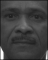
\includegraphics[scale=1.7]{f_h_images/AnyConv.com__00183_940128_fb}
                    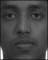
\includegraphics[scale=1.7]{f_h_images/AnyConv.com__00618_941031_fa}
                % \end{center}
                % \begin{center}
                    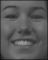
\includegraphics[scale=1.7]{f_h_images/AnyConv.com__00451_940422_fb}
                    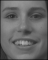
\includegraphics[scale=1.7]{f_h_images/AnyConv.com__00411_940422_fa}
                \end{center}
                \begin{center}
                    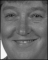
\includegraphics[scale=1.7]{f_h_images/AnyConv.com__00557_940519_fb}
                    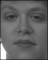
\includegraphics[scale=1.7]{f_h_images/AnyConv.com__00276_940422_fa}
                \end{center}
                \begin{center}
                    \scriptsize
                    Figure 10: Three query images and their incorrect matches from the \verb|fb_H| and \verb|fa_H| collections, respectively, with 90/95\% information
                    preservation.
                \end{center}

                Observing the CMC curve depicted in Figure 6, it would appear as if there is no significant difference between the identification accuracy. Similarly,
                the incorrect matches in Figures 8 and 10 seem relatively consistent; one can see the similarities between all presented matchings. We believe this may be
                because the high resolution images provide enough dimension to capture enough variance in the images within 80\% of the information. Overall, it would
                appear as the accuracy increases with the preserved data with the exception of the 95\%.

        \end{enumerate}

    \item[\textbf{b.}] When considering 50 subjects to be \textit{intruders}, we obtain the following ROC plot illustrated in Figure 11.
        \begin{center}
            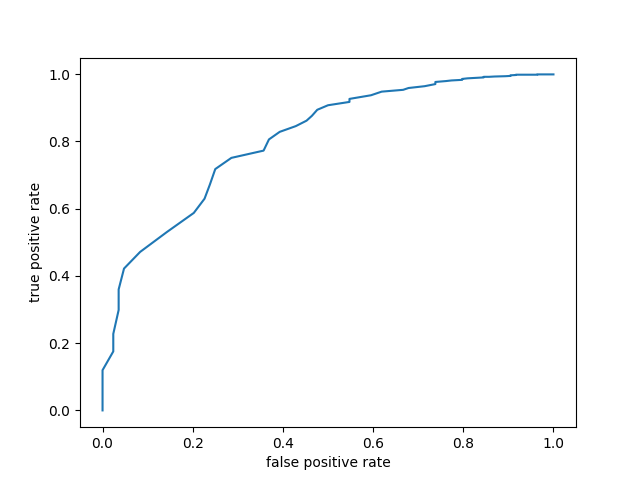
\includegraphics[scale=0.6]{roc_H}
        \end{center}
        \begin{center}
            \scriptsize
            Figure 11: The ROC curve for the \verb|fb_H| collection when considering intruders.
        \end{center}

    \item[\textbf{c.}]
        \begin{enumerate}
            \item[\textbf{i.}] The average face as well as the ten largest and smallest eigenfaces are presented in Figures 12, 13, and 14, respectively, for the \verb|fa_L| collection.
                \begin{center}
                    \includegraphics[scale=5]{AnyConv.com__average_face_2}
                \end{center}
                \begin{center}
                    \scriptsize
                    Figure 12: The average face of the \verb|fa_L| collection.
                \end{center}

                \begin{center}
                    \includegraphics[scale=5]{AnyConv.com__largest1_2}
                    \includegraphics[scale=5]{AnyConv.com__largest2_2}
                    \includegraphics[scale=5]{AnyConv.com__largest3_2}
                    \includegraphics[scale=5]{AnyConv.com__largest4_2}
                    \includegraphics[scale=5]{AnyConv.com__largest5_2}
                    \includegraphics[scale=5]{AnyConv.com__largest6_2}
                    \includegraphics[scale=5]{AnyConv.com__largest7_2}
                    \includegraphics[scale=5]{AnyConv.com__largest8_2}
                    \includegraphics[scale=5]{AnyConv.com__largest9_2}
                    \includegraphics[scale=5]{AnyConv.com__largest10_2}
                \end{center}
                \begin{center}
                    \scriptsize
                    Figure 13: The eigenfaces corresponding to the ten largest eigenvalues of the \verb|fa_L| collection.
                \end{center}

                \begin{center}
                    \includegraphics[scale=5]{AnyConv.com__smallest1_2}
                    \includegraphics[scale=5]{AnyConv.com__smallest2_2}
                    \includegraphics[scale=5]{AnyConv.com__smallest3_2}
                    \includegraphics[scale=5]{AnyConv.com__smallest4_2}
                    \includegraphics[scale=5]{AnyConv.com__smallest5_2}
                    \includegraphics[scale=5]{AnyConv.com__smallest6_2}
                    \includegraphics[scale=5]{AnyConv.com__smallest7_2}
                    \includegraphics[scale=5]{AnyConv.com__smallest8_2}
                    \includegraphics[scale=5]{AnyConv.com__smallest9_2}
                    \includegraphics[scale=5]{AnyConv.com__smallest10_2}
                \end{center}
                \begin{center}
                    \scriptsize
                    Figure 14: The eigenfaces corresponding to the ten smallest eigenvalues of the \verb|fa_L| collection.
                \end{center}
            \item[\textbf{ii.}] Figure 15 illustrates the CMC curve when varying the number of images with the highest similarity scores between 1 and 50.
                \begin{center}
                    \includegraphics[scale=0.6]{cmc_L}
                \end{center}
                \begin{center}
                    \scriptsize
                    Figure 15: The CMC curve for the \verb|fb_L| collection.
                \end{center}

            \item[\textbf{iii.}] Assuming that we consider only one image with the highest similarity score, Figure 16 illustrates query images and their corresponding correct matches
                when preserving 80\% of all information.
                \begin{center}
                    \includegraphics[scale=5]{f_l_images/AnyConv.com__00182_940422_fb_a}
                    \includegraphics[scale=5]{f_l_images/AnyConv.com__00182_940422_fa_a}
                % \end{center}
                % \begin{center}
                    \includegraphics[scale=5]{f_l_images/AnyConv.com__00753_941201_fb}
                    \includegraphics[scale=5]{f_l_images/AnyConv.com__00753_941201_fa}
                \end{center}
                \begin{center}
                    \includegraphics[scale=5]{f_l_images/AnyConv.com__00501_940519_fb}
                    \includegraphics[scale=5]{f_l_images/AnyConv.com__00501_940519_fa}
                \end{center}
                \begin{center}
                    \scriptsize
                    Figure 16: Three query images and their correct corresponding matches from the \verb|fb_L| and \verb|fa_L| collections, respectively, with 80\%
                    information preservation.
                \end{center}

            \item[\textbf{iv.}] Again, only considering only one image with the highest similarity score, Figure 17 depicts query images incorrectly matched when preserving 80\% of all
                information.
                \newpage
                \begin{center}
                    \includegraphics[scale=5]{f_l_images/AnyConv.com__00183_940128_fb}
                    \includegraphics[scale=5]{f_l_images/AnyConv.com__00716_941205_fa}
                % \end{center}
                % \begin{center}
                    \includegraphics[scale=5]{f_l_images/AnyConv.com__00451_940422_fb}
                    \includegraphics[scale=5]{f_l_images/AnyConv.com__00346_940422_fa}
                \end{center}
                \begin{center}
                    \includegraphics[scale=5]{f_l_images/AnyConv.com__00594_941031_fb}
                    \includegraphics[scale=5]{f_l_images/AnyConv.com__00383_941031_fa}
                \end{center}
                \begin{center}
                    \scriptsize
                    Figure 17: Three query images and their incorrect matches from the \verb|fb_L| and \verb|fa_L| collections, respectively, with 80\% information
                    preservation.
                \end{center}

            \item[\textbf{v.}] Now we repeat the process with 90\% and 95\% information preservation. Figures 18 and 19 illustrate three correct and incorrect matchings, respectively,
                with both 90\% data preservation. Similarly, Figures 20 and 21 represent the matchings with 95\% preservation.
                \begin{center}
                    \includegraphics[scale=5]{f_l_images/AnyConv.com__00182_940422_fb_a}
                    \includegraphics[scale=5]{f_l_images/AnyConv.com__00182_940422_fa_a}
                % \end{center}
                % \begin{center}
                    \includegraphics[scale=5]{f_l_images/AnyConv.com__00753_941201_fb}
                    \includegraphics[scale=5]{f_l_images/AnyConv.com__00753_941201_fa}
                \end{center}
                \begin{center}
                    \includegraphics[scale=5]{f_l_images/AnyConv.com__00501_940519_fb}
                    \includegraphics[scale=5]{f_l_images/AnyConv.com__00501_940519_fa}
                \end{center}
                \begin{center}
                    \scriptsize
                    Figure 18: Three query images and their correct corresponding matches from the \verb|fb_L| and \verb|fa_L| collections, respectively, with 90\%
                    information preservation.
                \end{center}
                \newpage

                \begin{center}
                    \includegraphics[scale=5]{f_l_images/AnyConv.com__00183_940128_fb}
                    \includegraphics[scale=5]{f_l_images/AnyConv.com__00276_940422_fa_a}
                % \end{center}
                % \begin{center}
                    \includegraphics[scale=5]{f_l_images/AnyConv.com__00451_940422_fb}
                    \includegraphics[scale=5]{f_l_images/AnyConv.com__00410_940422_fa}
                \end{center}
                \begin{center}
                    \includegraphics[scale=5]{f_l_images/AnyConv.com__00557_940519_fb}
                    \includegraphics[scale=5]{f_l_images/AnyConv.com__00002_940128_fa}
                \end{center}
                \begin{center}
                    \scriptsize
                    Figure 19: Three query images and their incorrect matches from the \verb|fb_L| and \verb|fa_L| collections, respectively, with 90\% information
                    preservation.
                \end{center}


                \begin{center}
                    \includegraphics[scale=5]{f_l_images/AnyConv.com__00182_940422_fb_a}
                    \includegraphics[scale=5]{f_l_images/AnyConv.com__00182_940422_fa_a}
                % \end{center}
                % \begin{center}
                    \includegraphics[scale=5]{f_l_images/AnyConv.com__00753_941201_fb}
                    \includegraphics[scale=5]{f_l_images/AnyConv.com__00753_941201_fa}
                \end{center}
                \begin{center}
                    \includegraphics[scale=5]{f_l_images/AnyConv.com__00501_940519_fb}
                    \includegraphics[scale=5]{f_l_images/AnyConv.com__00501_940519_fa}
                \end{center}
                \begin{center}
                    \scriptsize
                    Figure 20: Three query images and their correct corresponding matches from the \verb|fb_L| and \verb|fa_L| collections, respectively, with 95\%
                    information preservation.
                \end{center}
                \newpage

                \begin{center}
                    \includegraphics[scale=5]{f_l_images/AnyConv.com__00183_940128_fb}
                    \includegraphics[scale=5]{f_l_images/AnyConv.com__00618_941031_fa}
                % \end{center}
                % \begin{center}
                    \includegraphics[scale=5]{f_l_images/AnyConv.com__00451_940422_fb}
                    \includegraphics[scale=5]{f_l_images/AnyConv.com__00411_940422_fa}
                \end{center}
                \begin{center}
                    \includegraphics[scale=5]{f_l_images/AnyConv.com__00557_940519_fb}
                    \includegraphics[scale=5]{f_l_images/AnyConv.com__00276_940422_fa}
                \end{center}
                \begin{center}
                    \scriptsize
                    Figure 21: Three query images and their incorrect matches from the \verb|fb_L| and \verb|fa_L| collections, respectively, with 95\% information
                    preservation.
                \end{center}

                Now, notice that there is a separation within the identification accuracy as depicted in the CMC plot in Figure 15. Both the 90\% and 95\% converge to 1 at a faster
                rate than 80\%. We believe this is because the low resolution images may not provide enough dimensionality when considering only 80\% of information preservation.
                Overall, it would appear that more data preservation leads to higher accuracy.

        \end{enumerate}

    \item[\textbf{d.}] When considering 50 subjects to be intruders, we obtain the following ROC plot illustrated in Figure 22.
        \begin{center}
            \includegraphics[scale=0.6]{roc_L}
        \end{center}
        \begin{center}
            \scriptsize
            Figure 22: The ROC curve for the \verb|fb_L| collection when considering intruders.
        \end{center}

    \item[\textbf{e.}] When comparing the results between the low and high resolution images, it would appear as if the classifier performs almost equally well. It is true that the
        results from the low resolution collection had lower accuracy on average; however, with high information preservation, it would appear to have similar results to the
        high resolution images despite lack of definition. Our explanation for this outcome is that most facial information can still be extracted from a high data preservation of the
        low resolution images. That is, a high percentage of the variance within the data set is still captured in the low resolution images allowing the classifier to act nearly as
        proficient.


\end{enumerate}


\end{document}

